% -*- coding: utf-8 -*-
%-------------------------designed by zcf--------------
\documentclass[UTF8,a4paper,10pt]{ctexart}
\usepackage[left=3.17cm, right=3.17cm, top=2.74cm, bottom=2.74cm]{geometry}
\usepackage{amsmath}
\usepackage{graphicx,subfig}
\usepackage{float}
\usepackage{cite}
\usepackage{caption}
\usepackage{enumerate}
\usepackage{booktabs} %表格
\usepackage{multirow}
\usepackage{pythonhighlight}
\newcommand{\tabincell}[2]{\begin{tabular}{@{}#1@{}}#2\end{tabular}}  %表格强制换行
%-------------------------字体设置--------------
\usepackage{times} 
\newcommand{\yihao}{\fontsize{26pt}{36pt}\selectfont}           % 一号, 1.4 倍行距
\newcommand{\erhao}{\fontsize{22pt}{28pt}\selectfont}          % 二号, 1.25倍行距
\newcommand{\xiaoer}{\fontsize{18pt}{18pt}\selectfont}          % 小二, 单倍行距
\newcommand{\sanhao}{\fontsize{16pt}{24pt}\selectfont}  %三号字
\newcommand{\xiaosan}{\fontsize{15pt}{22pt}\selectfont}        % 小三, 1.5倍行距
\newcommand{\sihao}{\fontsize{14pt}{21pt}\selectfont}            % 四号, 1.5 倍行距
\newcommand{\banxiaosi}{\fontsize{13pt}{19.5pt}\selectfont}    % 半小四, 1.5倍行距
\newcommand{\xiaosi}{\fontsize{12pt}{18pt}\selectfont}            % 小四, 1.5倍行距
\newcommand{\dawuhao}{\fontsize{11pt}{11pt}\selectfont}       % 大五号, 单倍行距
\newcommand{\wuhao}{\fontsize{10.5pt}{15.75pt}\selectfont}    % 五号, 单倍行距
%-------------------------章节名----------------
\usepackage{ctexcap} 
\CTEXsetup[name={,、},number={ \chinese{section}}]{section}
\CTEXsetup[name={(,)},number={\chinese{subsection}}]{subsection}
\CTEXsetup[name={,.},number={\arabic{subsubsection}}]{subsubsection}
%-------------------------页眉页脚--------------
\usepackage{fancyhdr}
\pagestyle{fancy}
\lhead{\kaishu \leftmark}
% \chead{}
\rhead{\kaishu 机器学习实验报告}%加粗\bfseries 
\lfoot{}
\cfoot{\thepage}
\rfoot{}
\renewcommand{\headrulewidth}{0.1pt}  
\renewcommand{\footrulewidth}{0pt}%去掉横线
\newcommand{\HRule}{\rule{\linewidth}{0.5mm}}%标题横线
\newcommand{\HRulegrossa}{\rule{\linewidth}{1.2mm}}
%-----------------------伪代码------------------
\usepackage{algorithm}  
\usepackage{algorithmicx}  
\usepackage{algpseudocode}  
\floatname{algorithm}{Algorithm}  
\renewcommand{\algorithmicrequire}{\textbf{Input:}}  
\renewcommand{\algorithmicensure}{\textbf{Output:}} 
\usepackage{lipsum}  
\makeatletter
\newenvironment{breakablealgorithm}
  {% \begin{breakablealgorithm}
  \begin{center}
     \refstepcounter{algorithm}% New algorithm
     \hrule height.8pt depth0pt \kern2pt% \@fs@pre for \@fs@ruled
     \renewcommand{\caption}[2][\relax]{% Make a new \caption
      {\raggedright\textbf{\ALG@name~\thealgorithm} ##2\par}%
      \ifx\relax##1\relax % #1 is \relax
         \addcontentsline{loa}{algorithm}{\protect\numberline{\thealgorithm}##2}%
      \else % #1 is not \relax
         \addcontentsline{loa}{algorithm}{\protect\numberline{\thealgorithm}##1}%
      \fi
      \kern2pt\hrule\kern2pt
     }
  }{% \end{breakablealgorithm}
     \kern2pt\hrule\relax% \@fs@post for \@fs@ruled
  \end{center}
  }
\makeatother
%------------------------代码-------------------
\usepackage{xcolor} 
\usepackage{listings} 
\lstset{ 
breaklines,%自动换行
basicstyle=\small,
escapeinside=``,
keywordstyle=\color{ blue!70} \bfseries,
commentstyle=\color{red!50!green!50!blue!50},% 
stringstyle=\ttfamily,% 
extendedchars=false,% 
linewidth=\textwidth,% 
numbers=left,% 
numberstyle=\tiny \color{blue!50},% 
frame=trbl% 
rulesepcolor= \color{ red!20!green!20!blue!20} 
}
%------------超链接----------
\usepackage[colorlinks,linkcolor=black,anchorcolor=blue]{hyperref}
%------------------------TODO-------------------
\usepackage{enumitem,amssymb}
\newlist{todolist}{itemize}{2}
\setlist[todolist]{label=$\square$}
% for check symbol 
\usepackage{pifont}
\newcommand{\cmark}{\ding{51}}%
\newcommand{\xmark}{\ding{55}}%
\newcommand{\done}{\rlap{$\square$}{\raisebox{2pt}{\large\hspace{1pt}\cmark}}\hspace{-2.5pt}}
\newcommand{\wontfix}{\rlap{$\square$}{\large\hspace{1pt}\xmark}}
%------------------------水印-------------------
\usepackage{tikz}
\usepackage{xcolor}
\usepackage{eso-pic}

\newcommand{\watermark}[3]{\AddToShipoutPictureBG{
\parbox[b][\paperheight]{\paperwidth}{
\vfill%
\centering%
\tikz[remember picture, overlay]%
  \node [rotate = #1, scale = #2] at (current page.center)%
    {\textcolor{gray!80!cyan!30!magenta!30}{#3}};
\vfill}}}



%———————————————————————————————————————————正文———————————————————————————————————————————————
%----------------------------------------------
\begin{document}
\begin{titlepage}
    \begin{center}
    
\includegraphics[width=0.8\textwidth]{NKU.png}\\[1cm]    
    \textsc{\Huge \kaishu{\textbf{南\ \ \ \ \ \ 开\ \ \ \ \ \ 大\ \ \ \ \ \ 学}} }\\[0.9cm]
    \textsc{\huge \kaishu{\textbf{计\ \ 算\ \ 机\ \ 学\ \ 院}}}\\[0.5cm]
    \textsc{\Large \textbf{机器学习实验报告}}\\[0.8cm]
    \HRule \\[0.9cm]
    { \LARGE \bfseries 实验四\ 层次聚类}\\[0.4cm]
    \HRule \\[2.0cm]
    \centering
    \textsc{\LARGE \kaishu{姓名\ :\ 王泳鑫}}\\[0.5cm]
    \textsc{\LARGE \kaishu{学号\ :\ 1911479}}\\[0.5cm]
    \textsc{\LARGE \kaishu{年级\ :\ 2019级}}\\[0.5cm]
    \textsc{\LARGE \kaishu{专业\ :\ 计算机科学与技术}}\\[0.5cm]
    \textsc{\LARGE \kaishu{指导教师\ :\ 卫金茂}}\\[0.5cm]
    \vfill
    {\Large \today}
    \end{center}
\end{titlepage}
%-------------摘------要--------------
\newpage
\thispagestyle{empty}
\renewcommand{\abstractname}{\kaishu \sihao \textbf{摘要}}
    \begin{abstract}

        \noindent  %顶格
        \textbf{\\\ 关键字:层次聚类,Machine Learning , Deep Learning}\textbf{} \\\ \\\
    \end{abstract}
%----------------------------------------------------------------
\tableofcontents
%----------------------------------------------------------------
\newpage
\watermark{60}{10}{NKU}
\setcounter{page}{1}
%——————————————————————————————————————
\section{实验描述与要求}
数据集:生成2000个样例,每个样例的前3列表示特征,第四列表示标签

基本要求:绘制聚类前后样本分布情况

\begin{enumerate}
    \item 实现single-linkage层次聚类算法;
    \item 实现complete-linkage层次聚类算法。
\end{enumerate}

中级要求:实现average-linkage层次聚类算法,绘制样本分布图。

提高要求:对比上述三种算法,给出结论。

%----------------------------------------------------------------
\section{程序设计与代码实现}
首先,我们还是要使用lab3中生成数据集的函数来生成本次实验的数据集,只不过我们需要进行一些修改,
每个样例由三个特征,和一个label,所以是四维的样例。但是我们可以借助一些sklearn中的函数,make\_blobs方法就是一个
专门为聚类产生数据集的方法,可以产生一个数据相应的标签,我们要对产生时的标签进行保存,以保证后面验证正确率的逻辑正确性。

我们实现聚合聚类的方法就是通过计算欧式距离,代码如下:

\begin{python}
def cal_node_distance(node1, node2):
    return np.sqrt(np.sum(np.square(node1 - node2)))  # 计算欧式距离

def cal_set_distance(set1, set2, method):
    dists = []  #初始化距离矩阵
    #遍历两个类的每一个样例,并且计算两个样例之间的欧氏距离,存入dists中
    for i in range(set1.shape[0]):
        cur1 = set1[i]
        for j in range(set2.shape[0]):
            cur2 = set2[j]
            dist = cal_node_distance(cur1, cur2)
            dists.append(dist)
    #不同的方法对两个类中欧氏距离的要求不同
    if method is 'single':
        return np.min(dists)  #最短距离
    elif method is 'complete':
        return np.max(dists)  #最长距离
    elif method is 'average':
        return np.mean(dists) #平均距离
    else:
        raise IOError('Illegal method')
\end{python}

然后就是我们的聚合聚类操作方法,这里以average-linkage层次聚类算法为例,single-linkage和complete-linkage算法都与其相似,代码如下:

\begin{python}
def average_linkage_clustering(sample, k):
    clusters = []   #初始化聚类
    for i in range(sample.shape[0]):
        node = []
        node.append(i)
        clusters.append(node)
    dists_matrix = []
    for i in range(len(clusters)):
        dists = []
        cur_set1 = sample[clusters[i]]
        for j in range(len(clusters)):
            cur_set2 = sample[clusters[j]]
            dist = cal_set_distance(cur_set1, cur_set2, method='average')
            dists.append(dist)
        dists_matrix.append(dists)
    dists_matrix = np.array(dists_matrix)
    while len(clusters) != k:  #当簇没有到我们要求的k个时,停止聚合聚类。
        base_idx = np.argmin(np.min(dists_matrix, 1))
        base_dist = dists_matrix[base_idx]
        target_idx = np.argsort(base_dist)[1]
        for each in clusters[target_idx]:
            clusters[base_idx].append(each)
        del clusters[target_idx]
        dists_matrix = np.delete(dists_matrix, target_idx, axis=0)
        dists_matrix = np.delete(dists_matrix, target_idx, axis=1)
        if base_idx > target_idx:
            base_idx -= 1
        for i in range(len(clusters)):
            dists_matrix[base_idx, i] = cal_set_distance(sample[clusters[base_idx]],sample[clusters[i]], method='average')
            dists_matrix[i, base_idx] = dists_matrix[base_idx, i]
    return clusters, dists_matrix
\end{python}

然后对聚类聚合计算的结果进行正确率的计算,通过使用一开始生成数据集的正确标签和最后聚合聚类的簇进行比对,代码如下:

\begin{python}
def cal_acc(pred, true):
    correct = 0
    for i in range(pred.shape[0]):
        if pred[i] == true[i]:
            correct += 1
    return correct/pred.shape[0]
\end{python}

最后,我们通过结果分析函数对最后预测的结果,把0、1、2、3四种标签的排列情况依次遍历,然后再选出正确率最高的
标签作为预测标签,然后返回正确率和预测标签,返回预测标签方便通过散点的形式表示出来,代码如下:

\begin{python}
def result_analysis(sample, label, k, method='average'):
    '''结果分析接口'''
    if method == 'single':
        clusters, dists_matrix = single_linkage_clustering(sample, k)
    elif method == 'average':
        clusters, dists_matrix = average_linkage_clustering(sample, k)
    elif method == 'complete':
        clusters, dists_matrix = complete_linkage_clustering(sample, k)
    accs = []
    pred_labels = []
    cases = [x for x in range(k)]
    cases = permutations(cases) # 0、1、2、3四种标签的排列情况
    for case in cases:
        pred_label = np.zeros(label.shape)#首先创建一个零矩阵
        for i in range(case.__len__()):#依次遍历
            pred_label[clusters[i]] = case[i]
        pred_labels.append(pred_label)
        acc = cal_acc(pred_label, label)
        accs.append(acc)
    acc = np.max(accs) # 将排列中准确度最高的情况作为预测标签
    pred_label = pred_labels[np.argmax(accs)]
    return acc, pred_label

\end{python}

\section{结果演示与分析}

首先,我们可以通过plot来展示我们随机生成的数据集的散点图,如图\ref{fig:1}所示
\begin{figure}[H]
    \centering
    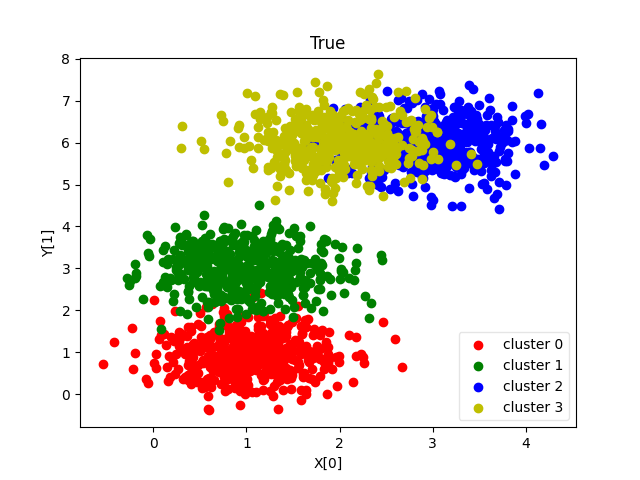
\includegraphics[scale=0.7]{1.png}
    \caption{数据集}
    \label{fig:1}
\end{figure}

如图\ref{fig:1}所示,我们可以看到single-linkage的聚合聚类的结果。

\begin{figure}[H]
    \centering
    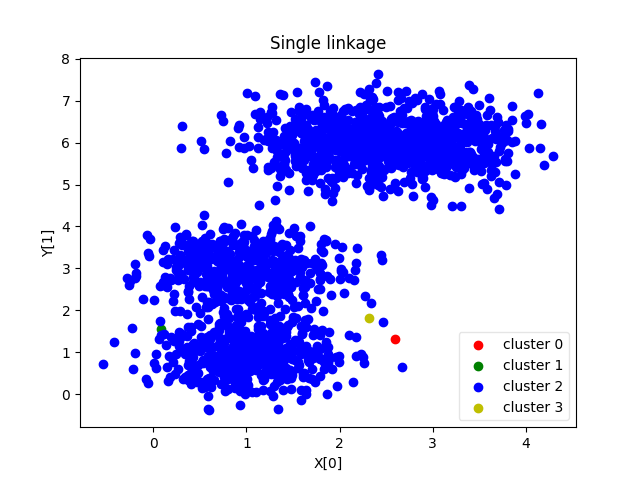
\includegraphics[scale=0.7]{2.png}
    \caption{single-linkage}
    \label{fig:1}
\end{figure}

如图\ref{fig:1}所示,我们可以看到average-linkage的聚合聚类的结果。

\begin{figure}[H]
    \centering
    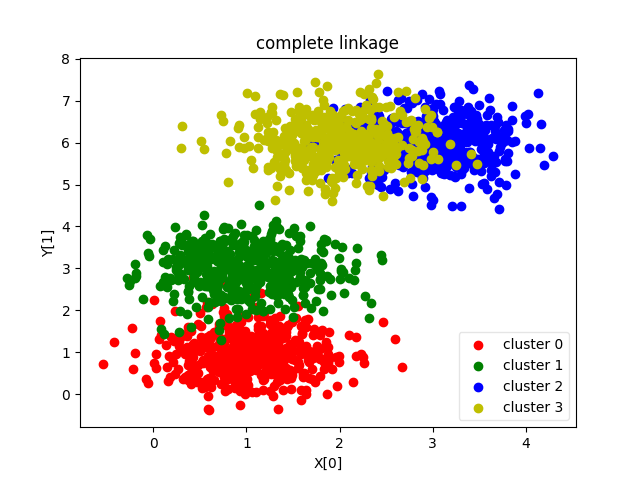
\includegraphics[scale=0.7]{3.png}
    \caption{average-linkage}
    \label{fig:1}
\end{figure}


如图\ref{fig:1}所示,我们可以看到complete-linkage的聚合聚类的结果。

\begin{figure}[H]
    \centering
    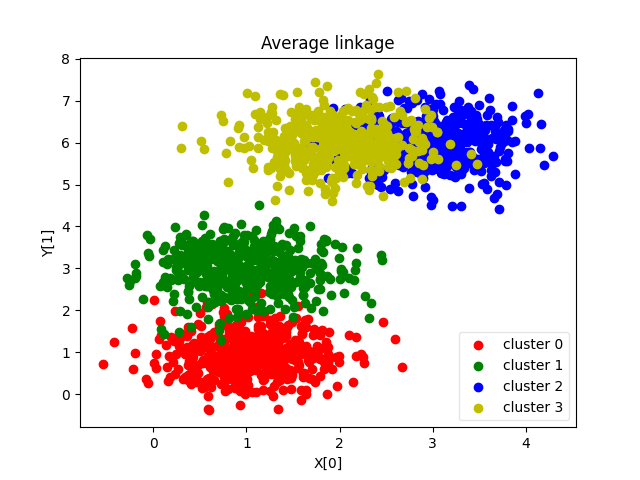
\includegraphics[scale=0.7]{4.png}
    \caption{complete-linkage}
    \label{fig:1}
\end{figure}

根据上面三幅图展示的结果,我们可以看到average-linkage和complete-linkage这两种聚合聚类算法最后预测的结果都是不错的,
相较于single-linkage聚合聚类算法正确率更高,具体的正确率如图\ref{fig:1}所示:

\begin{figure}[H]
    \centering
    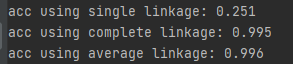
\includegraphics[scale=0.7]{5.png}
    \caption{正确率}
    \label{fig:1}
\end{figure}

为了对比上述三种算法的效果,我改变了k的大小来探究不同算法在k值为多少时最优,以及随k值变化算法效果变化的浮动,结果如图\ref{fig:1}所示:

\begin{figure}[H]
    \centering
    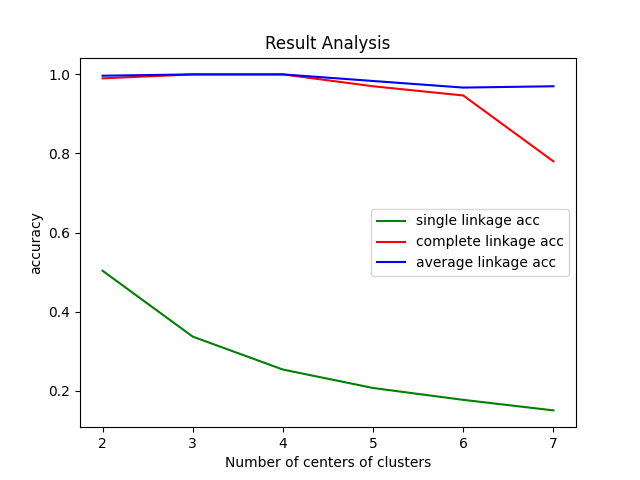
\includegraphics[scale=0.7]{6.png}
    \caption{准确率变化}
    \label{fig:1}
\end{figure}

我们可以发现随着k值的变化,single-linkage的准确率变化在慢慢减小,最后甚至低于0.2的准确率,complete-linkage算法一开始保持一个比较高的准确率,但是随着k值的增加准确率开始下降,当k=7时,准确率降到了0.8以下。相比之下,
average-linkage算法的准确率一直都保持在一个比较高的状态。

%----------------------------------------------------------------
\bibliographystyle{plain}
\end{document}
